%!TEX root = mb.tex

\section{Evaluation} \label{sec:eval}

As we showed in \S\ref{sec:impl}, \sys supports all middlebox applications in typical outsourcing environments~\cite{aplomb,nfv} -- including header-only middleboxes (which \sys supports without modification) as well as DPI middleboxes (which \sys supports with modifications to their codebase). 
Hence, from a functionality perspective, \sys answers our original question, ``Is it possible to enable a third party to perform traffic processing for an enterprise, {\em without seeing the enterprise's traffic}?''  strongly in the affirmative.

To evaluate \sys more deeply, we now try to get a sense whether \sys is practical from a performance perspective, looking at the overheads due to encryption at (a) the gateway, and (b) the middleboxes themselves. Overall, we find that \sys with no DPI reduces gatway throughput by \todo{foo\%} and has zero overhead at the outsourced middleboxes. \sys with DPI enabled imposes a higher overhead, with the gateway throughput reduced by \todo{bar\%} and typical middlebox throughput reduced to \todo{baz\%} of baseline. 

\todo{methodology, datasets...}

\subsection{Gateway and MB Throughput}
We first provide some high-level throughput figures illustrating the overheads at the gatway and the middleboxes; in the following subsections we investigate the performance properties of each appliance in detail.

\begin{figure}[t]
  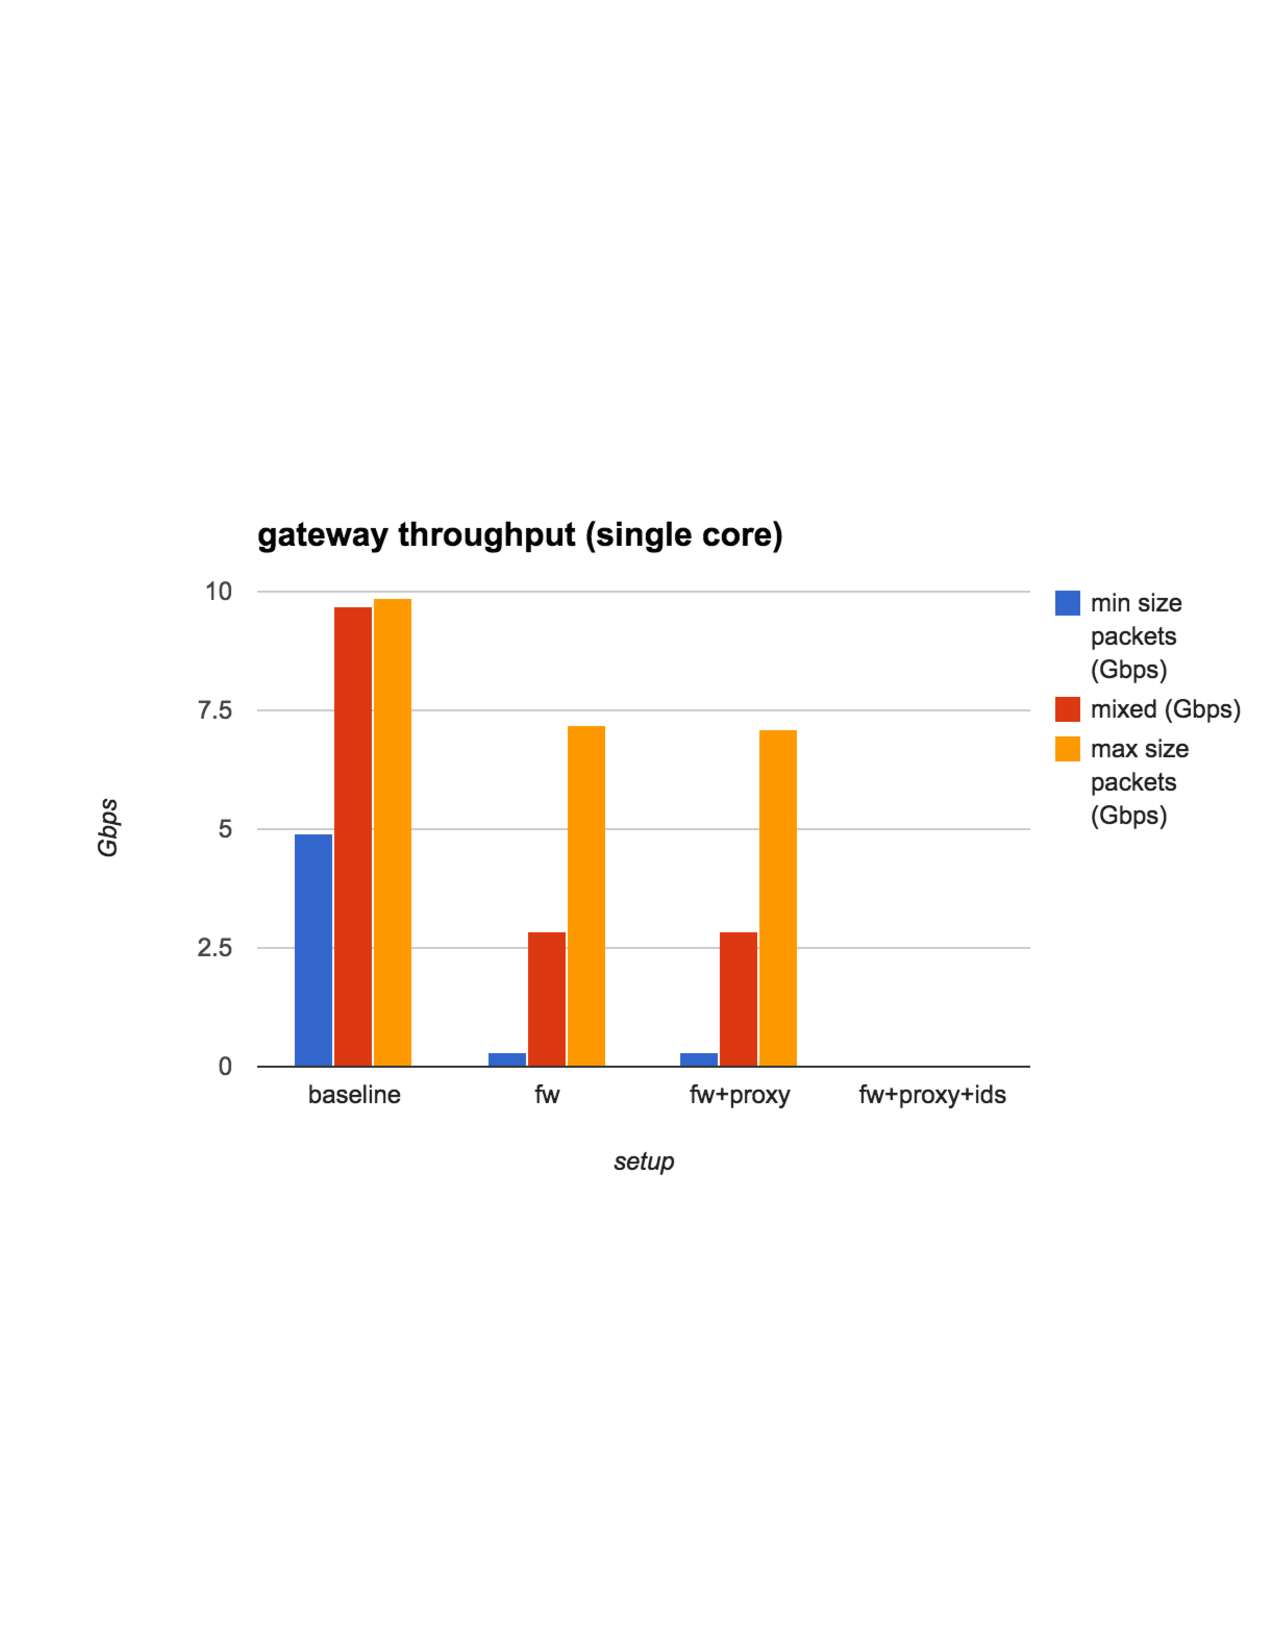
\includegraphics[width=3in]{fig/gatewayxput}
  \caption[]{\label{fig:gwxput} Throughput at the gateway without \sys, with header-only \sys, with HTTP-aware \sys, and with DPI-enabled \sys.}
\end{figure}


\noindent{\it How does encryption impact throughput at the outsourcing gateway relative to an outsourcing gateway without \sys?}
Figure~\ref{fig:gwxput}...


\begin{table}[t!]
\begin{tabular}{p{2.5cm}|p{1.4cm}|p{2cm}|p{1cm}}
Application & Header / HTTP / DPI & Baseline xput & \sys xput \\
\hline \hline
IP Firewall &   &  &  \\
Application Firewall & & & \\
NAT & Yes  & &  \\
IP Forwarding & & & \\
VPN Gateway &  &  &  \\ 
Load Balancer L4 & & & \\
Load Balancer L7 & & & \\
WAN optimizer  & & & \\
Web proxy/cache forward/ reverse & & &\\
IDS & & & \\
Exfiltration/parental filtering & & &  \\
\todo{split this} 
\end{tabular}
\caption{Middlebox applications supported by \sys and their throughput with an emprical traffic workload. \label{tbl:appsxput}}
\end{table}

\noindent{\it Is throughput reduced at the middleboxes due to \sys?}
(Hopefully we can say, for most apps, not at all)
Table~\ref{tbl:appsxput}...

\subsection{In Detail: The Gateway}

\begin{figure}[t]
  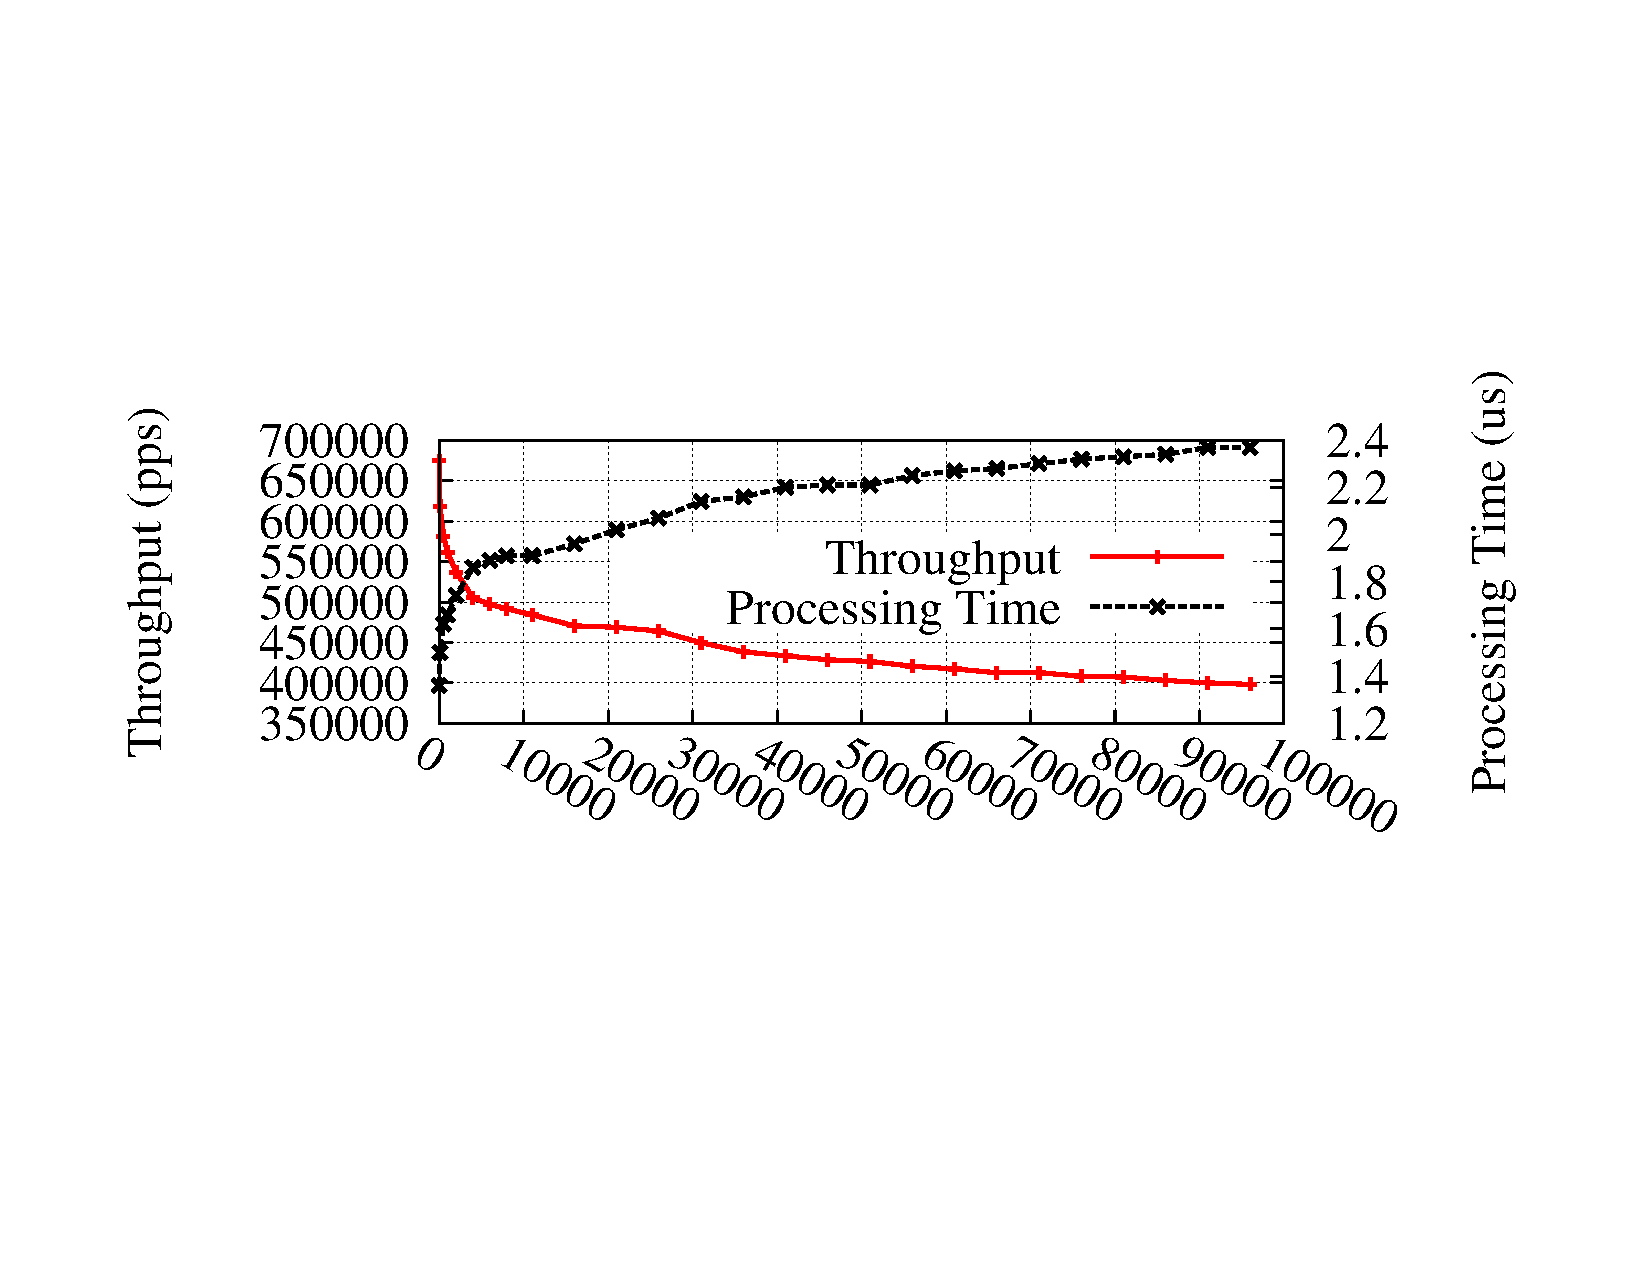
\includegraphics[width=3in]{fig/xputrange}
  \caption[]{\label{fig:xputrange} Throughput as number of rules for range encrypt increases.}
\end{figure}


\begin{figure}[t]
  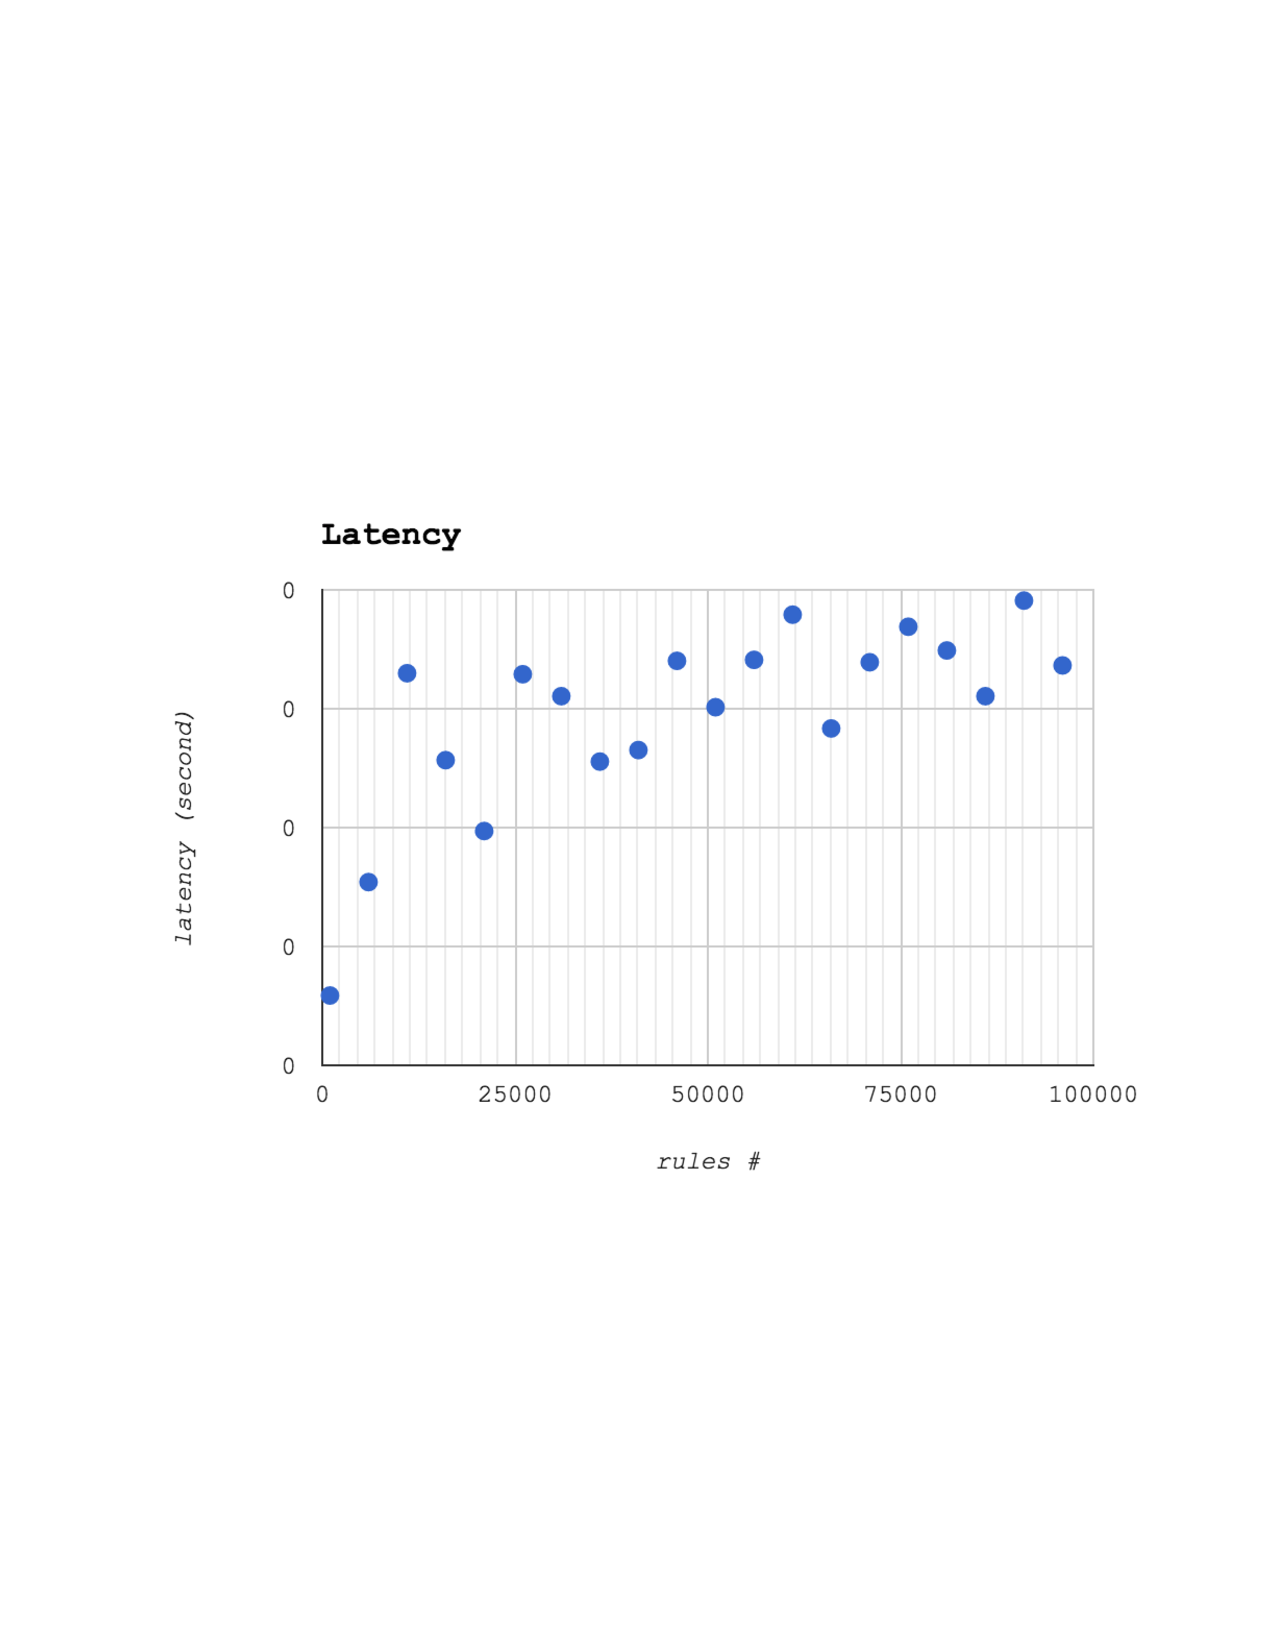
\includegraphics[width=3in]{fig/latencyrange}
  \caption[]{\label{fig:latencyrange} Per-packet latency as number of rules for range encrypt increases.}
\end{figure}


\noindent{\it How do throughput and latency scale with the number of rules for range encryption?} 
Figs~\ref{fig:latencyrange} and~\ref{fig:xputrange}

\noindent{\it What is the memory overhead of the stateful range map encryption scheme?}

\noindent{\it How much does border packet encoding increase throughput relative to flow reconstruction?}

\noindent{\it How much does bandwidth from the gateway to the cloud increase due to IPv4 to v6 conversion? Due to HTTP or DPI encryption?}

\subsection{In Detail: Header-Only Middleboxes}

\noindent{\bf Firewalls.} {\it Does \sys support all rules in a typical firewall configuration? How much does the ruleset ``expand'' due to encryption?}

\noindent{\it How often do updates to the firewall require a rule refresh? How long does it take to refresh rules at the firewall?}

\noindent{\bf NAT.}
\noindent{\bf LB...}

\subsection{In Detail: DPI Middleboxes}

\noindent{\bf Proxy/Caching.}
{\it How many active connections per second can the Proxy accept? How does this compare to an unencrypted Proxy implementation, like Squid?}

{\it What improvement in page load times does a client experience due to proxying, relative to no proxy at all? Relative to an unencrypted proxy implementation?}

\noindent{\bf Intrusion Detection}
{\it How much does MBArk reduce flow completion times relative to BlindBox~\cite{blindbox}?}

{\it How fast is detection time (with border encrypt) relative to BlindBox (without border encrypt)?}

\eat{
\todo{do we want to have a section on whether it changes the processing at the middlebox? 
perhaps also a discussion
of how easy it is to setup/configure/admin support for gateway?}

microbenchmark boundary encryption, IDS encryption, range match, equality

\subsection{Functionality}

Table~\ref{tab:apps} lists the various applications supported in the APLOMB model~\cite{aplomb} 
and whether \sys supports them. 

\todo{make sure this does not duplicate intro table}

\todo{L4 firewall vs the other firewalls}
\todo{some notes on this table from talking to Justine -- e.g., add what needs to be modified; also add what operations each uses}
cannot support reverse proxy and wan optimization -- explain why -- also these are causing problems to aplomb that some consider not even putting on cloud 


Table for IDS:

\begin{table}[t]
  \centering
  \begin{tabular}{l|c|c}
    {\bf Dataset}&{\bf SEC I.}&{\bf SEC II.}\\
    \hline
    Document Watermarking~\cite{CMU_exfiltration_report}&100\%&100\%\\
    \hline
    Snort Community (HTTP)&\twosnortcom&100\%\\
    \hline
    Snort Emerging Threats (HTTP)&\twosnortemerge&100\%\\
    \hline
    StoneSoft (McAffee) IDS&40\%&100\%\\
    \hline
    LastLine IDS&29.1\%&100\%\\
  \end{tabular}
  \caption[]{\label{tbl:coverage} Fraction of attack signatures in public and industrial signature\
 sets addressable with security guarantees I and II explained in \S\ref{sec:BB} \label{tab:BB_sec_func}. }
\end{table}




\subsection{Performance evaluation}

}
